% Packages & Document Configurations
\documentclass[twocolumn]{NobArticle}
\runninghead{Shortened Running Article Title}
\footertext{\textit{Journal X} (2023) 12:684}

\usepackage{import}

% Title
\title{Incompressible Fluid Simulation: A Comparison}

% Authors
\author{
    YUMENG HE, University of Southern California, USA \\
    HSIN LI, University of Southern California, USA \\
    YUCHEN CHEN, University of Southern California, USA \\
    XU CHEN, University of Southern California, USA
}

% Abstract
\renewcommand{\maketitlehookd}{%
\begin{abstract}
    \noindent Our project is a 2D incompressible fluid simulation implemented in C++ with visualization using OpenGL and GLUT. The main objective is to compare the performance, visual behavior, and numerical characteristics of different fluid simulation methods, including: Grid-based (Stable Fluids), Particle-based (SPH), Particle-In-Cell (PIC),hybrid PIC/FLIP method(PIC/FLIP), Affine Particle-In-Cell (APIC)
    This simulation provides a visual and algorithmic comparison of each method's strengths and weaknesses.
    
    \medskip

    \small{\textbf{Index Terms:} fluid simulation, incompressible, particle, grid, hybird}
\end{abstract}
}

\begin{document}

\small
\maketitle

% Introduction
\section{Introduction}

Fluid simulation is a central topic in physics-based graphics and engineering.
Researchers study two broad classes of flow.
Compressible fluids—such as smoke, fire, or drifting snow—change density as they move.
Incompressible fluids—such as water—preserve volume.
Our project narrows its focus to incompressible flow because it underpins many game and film effects.

Scientists have pursued fluid solvers for more than three decades.
Early work in the 1990 s split along two lines. Grid-based methods stored velocity on fixed cells and solved pressure on a lattice.
Particle methods—notably Smoothed Particle Hydrodynamics (SPH)—tracked discrete parcels of mass.
Each line had limits: grids diffused small details, while pure particles struggled with volume loss and boundary handling.

Around 2000, hybrid techniques emerged.
Particle-In-Cell (PIC) used a grid for forces and particles for advection.
FLIP kept the same layout but reduced numerical damping.
Material Point Method (MPM) added elastoplastic behavior for snow-like media.
Affine Particle-In-Cell (APIC) later improved rotational fidelity by carrying local affine velocity.
These methods mix Eulerian and Lagrangian views to balance stability and detail.

Our project builds an interactive framework that implements five representatives: Stable Fluids (grid), SPH (particle), PIC, hybrid PIC/FLIP, and APIC.
We run every solver on the same domain, time step, and boundary conditions. We then measure speed, memory use, and visual artifacts.
The side-by-side view reveals each method's trade-off between diffusion, noise, and stability, and helps artists choose the right tool for a desired effect.


% Contribution
\subsection{Contribution}
This project as the follow contributions.
\begin{itemize}
	\item The codebase supports five fluid solvers behind one interface. Users can swap methods with a single flag.
	\item The viewer renders density, velocity, and vorticity in real time. It uses GLUT for portability.
	\item We fix domain size, time step, and boundary conditions across all tests. This isolates algorithmic differences.
	\item We capture signature phenomena such as diffusion, particle clumping, and energy drift. Screenshots and videos illustrate each effect.
\end{itemize}

\section{Background}
Fluid simulation typically relies on solving the Navier-Stokes equations, which describe fluid motion as follows:
\begin{equation}
\frac{\partial \mathbf{u}}{\partial t} + (\mathbf{u}\cdot\nabla)\mathbf{u} = -\frac{1}{\rho}\nabla p + \nu\nabla^2\mathbf{u} + \mathbf{f}
\end{equation}
\begin{equation}
\nabla \cdot \mathbf{u} = 0
\end{equation}
where $\mathbf{u}$ is the velocity field, $p$ is the pressure, $\rho$ is the density, $\nu$ is the kinematic viscosity, and $\mathbf{f}$ represents external forces like gravity or user input. The second equation enforces incompressibility.

\subsection{Grid-based (Stable Fluids)}
Grid-based methods store velocity and pressure fields on a fixed Eulerian grid. The Stable Fluids method proposed by Stam \citet{Stam 1999} employs an implicit numerical scheme that guarantees stability at the cost of numerical diffusion. This approach involves four primary steps: advection, diffusion, force application, and pressure projection to ensure incompressibility. Although easy to implement and stable, this method diffuses small-scale features rapidly, causing loss of detail.

\subsection{Particle-based (SPH)}
Smoothed Particle Hydrodynamics (SPH) is a purely Lagrangian, particle-based technique. It represents fluid with discrete particles that carry fluid properties such as density and velocity \cite{Monaghan1992SPH}. Particle interactions are computed using smoothing kernels, enabling flexible boundary handling and adaptive resolution. However, SPH often struggles with preserving volume and can produce noisy visual artifacts, especially with low particle counts.

\subsection{Hybrid Methods}
Hybrid approaches blend Eulerian grids and Lagrangian particles, seeking a balance between stability, accuracy, and visual realism. Notable hybrid methods include:

\textbf{Particle-In-Cell (PIC)}: PIC \cite{Harlow1964PIC} transfers velocities from particles to a grid to compute pressure and forces, then advects particles using the grid velocities. It offers stability but introduces significant numerical damping.

\textbf{FLuid Implicit Particle (FLIP)}: An improvement over PIC, FLIP \cite{Brackbill1986FLIP} reduces numerical damping by transferring velocity changes, rather than absolute velocities, from grid to particles.

\textbf{Affine Particle-In-Cell (APIC)}: APIC \cite{Jiang2015APIC} further improves rotational and detailed motion preservation by storing affine velocity transformations for each particle, mitigating excessive dissipation seen in PIC/FLIP methods.

\textbf{Material Point Method (MPM)}: Extending PIC, MPM \cite{Sulsky1995MPM} simulates elastoplastic and granular materials by integrating material deformation through particle-grid interactions. 

Other advanced hybrid variations include:
\begin{itemize}
\item \textbf{PolyPIC} \cite{Fu2017PolyPIC}, which uses polynomial velocity reconstruction to reduce numerical dissipation.
\item \textbf{MLS-MPM} (Moving Least Squares MPM) \cite{Hu2018MLSMPM}, enhancing accuracy by employing MLS interpolation.
\item \textbf{Impulse PIC} \cite{Jiang2021ImpulsePIC}, improving collision handling by explicitly resolving impulses at boundaries.
\end{itemize}
These hybrid methods significantly advance fluid simulation, enabling realistic visualization with reduced artifacts and increased computational stability.
\section{Methods}
To accomplish our project goals, we implemented five distinct 2D incompressible fluid simulation methods—Stable Fluids, SPH, PIC, PIC/FLIP, and APIC—using C++ for the core simulation and OpenGL with GLUT for real-time visualization. Each method was developed independently based on its underlying physical principles and algorithmic structure. We focused on observing and comparing the visual behavior and numerical characteristics of each simulation through qualitative analysis. The following sections describe the implementation details and key observations for each method.

\textbf{Tools and Learning} We used C++ for simulation logic and OpenGL with GLUT for real-time visualization across all simulation methods. The Eigen library was employed for efficient matrix operations, particularly for APIC and FLIP methods where affine velocity matrices were involved. 

Throughout the project, we learned how to structure particle-grid transfer systems, implement spatial neighborhood queries using a sorting grid, and visualize thousands of particles in real time. We also gained practical experience with parallel programming, numerical debugging, and enforcing boundary conditions on staggered MAC grids.

\textbf{Course Content Reference} We applied key concepts from the course, including hybrid fluid simulation methods (PIC, FLIP, APIC), particle-grid transfers, SPH kernel functions, external forces, and pressure projection. These topics directly guided our simulation and implementation strategy.

% \begin{figure}[!htpb]
%     \centering
%     \includegraphics[width=\linewidth]{Figures/PezizaTuberosa.jpg}
%     \caption{Illustration of the fungus Dumontinia tuberosa by physician, mycologist, and illustrator Charles Tulasne (1816–1884) in the book Selecta Fungorum Carpologia (1861–65). (Name of the original work: Peziza tuberosa parasite on Anemone nemorosa).}
%     \label{fig:tcanther}
% \end{figure}

grid
\subsection{Particle}
We used a particle fluid simulation method proposed by Müller \cite{Muller2003} based on Smoothed Particle Hydrodynamics (SPH).

\subsection{PIC}

The Particle-In-Cell (PIC) method uses both particles and grids for fluid simulation. Each simulation step involves five primary phases:

\begin{enumerate}
\item \textbf{Transfer to Grid}: Particle velocities are transferred to nearby grid cells using B-spline weighting functions.
The compact quadratic B-spline kernel used is:
\begin{equation}
w(r) =
\begin{cases}
0.75 - r^2, & 0 \le r < 0.5 \\
0.5 \cdot (1.5 - r)^2, & 0.5 \le r < 1.5 \\
0, & \text{otherwise}
\end{cases}
\end{equation}

\item \textbf{Apply Gravity}: Gravity force is applied directly to vertical grid velocities.
Grid velocity is updated using:
\begin{equation}
\vec{v}_{i,j}.y \mathrel{-}= g \cdot \Delta t
\end{equation}

\item \textbf{Solve Pressure}: The pressure Poisson equation is solved using Jacobi iteration. Initially, divergence is calculated for each grid cell. 
\begin{equation}
  \nabla \cdot \vec{v}_{i,j} = \frac{v_{i+1,j}.x - v_{i-1,j}.x}{2} + \frac{v_{i,j+1}.y - v_{i,j-1}.y}{2}
  \end{equation}

Then, pressure values are iteratively adjusted to minimize divergence, enforcing incompressibility.
\begin{equation}
  p_{i,j}^{(k+1)} = \frac{1}{N} \left( \sum_{\text{fluid neighbors}} p^{(k)} - \nabla \cdot \vec{v}_{i,j} \right)
  \end{equation}
  where \( N \) is the number of neighboring fluid cells.

The velocity field is updated by subtracting the pressure gradient.
\begin{equation}
  \vec{v}_{i,j}.x \mathrel{-}= \frac{p_{i+1,j} - p_{i-1,j}}{2}, \quad
  \vec{v}_{i,j}.y \mathrel{-}= \frac{p_{i,j+1} - p_{i,j-1}}{2}
  \end{equation}

\item \textbf{Transfer Back to Particles}: Updated grid velocities are interpolated back onto particles.
\begin{equation}
  \vec{v}_p = \sum_{(i,j)} w_{(i,j) \rightarrow p} \cdot \vec{v}_{i,j}
  \end{equation}

\item \textbf{Move Particles}: Particles are advected according to their updated velocities. Boundary conditions are enforced by repositioning particles inside the domain and setting boundary normal velocities to zero.
\begin{equation}
  \vec{x}_p \mathrel{+}= \vec{v}_p \cdot \Delta t
  \end{equation}
\end{enumerate}

\subsubsection{Intermediate Results and Diagrams (PIC)}

In the Figure~\ref{fig:pic}, the \textbf{yellow arrows} show the grid velocity at some grid points.

\begin{figure*}[h]
  \centering
  \begin{subfigure}[t]{0.2\textwidth}
      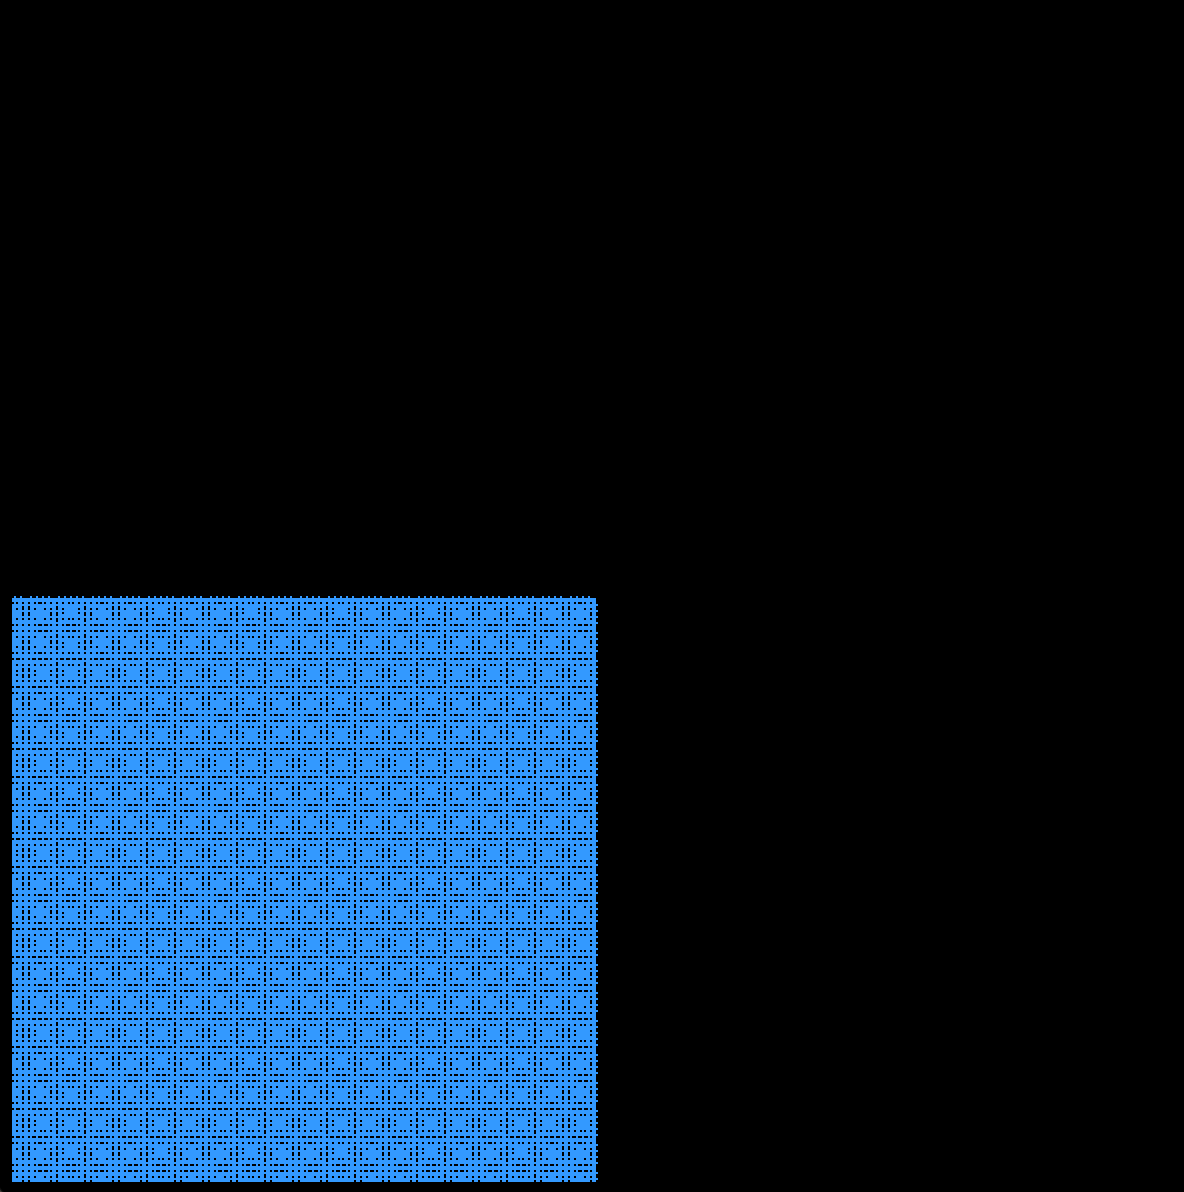
\includegraphics[width=\textwidth]{figures/pic_init.png}
      \caption{Initially, all particles are in the bottom-left corner.}
  \end{subfigure}
  \hspace{1em}
  \begin{subfigure}[t]{0.2\textwidth}
      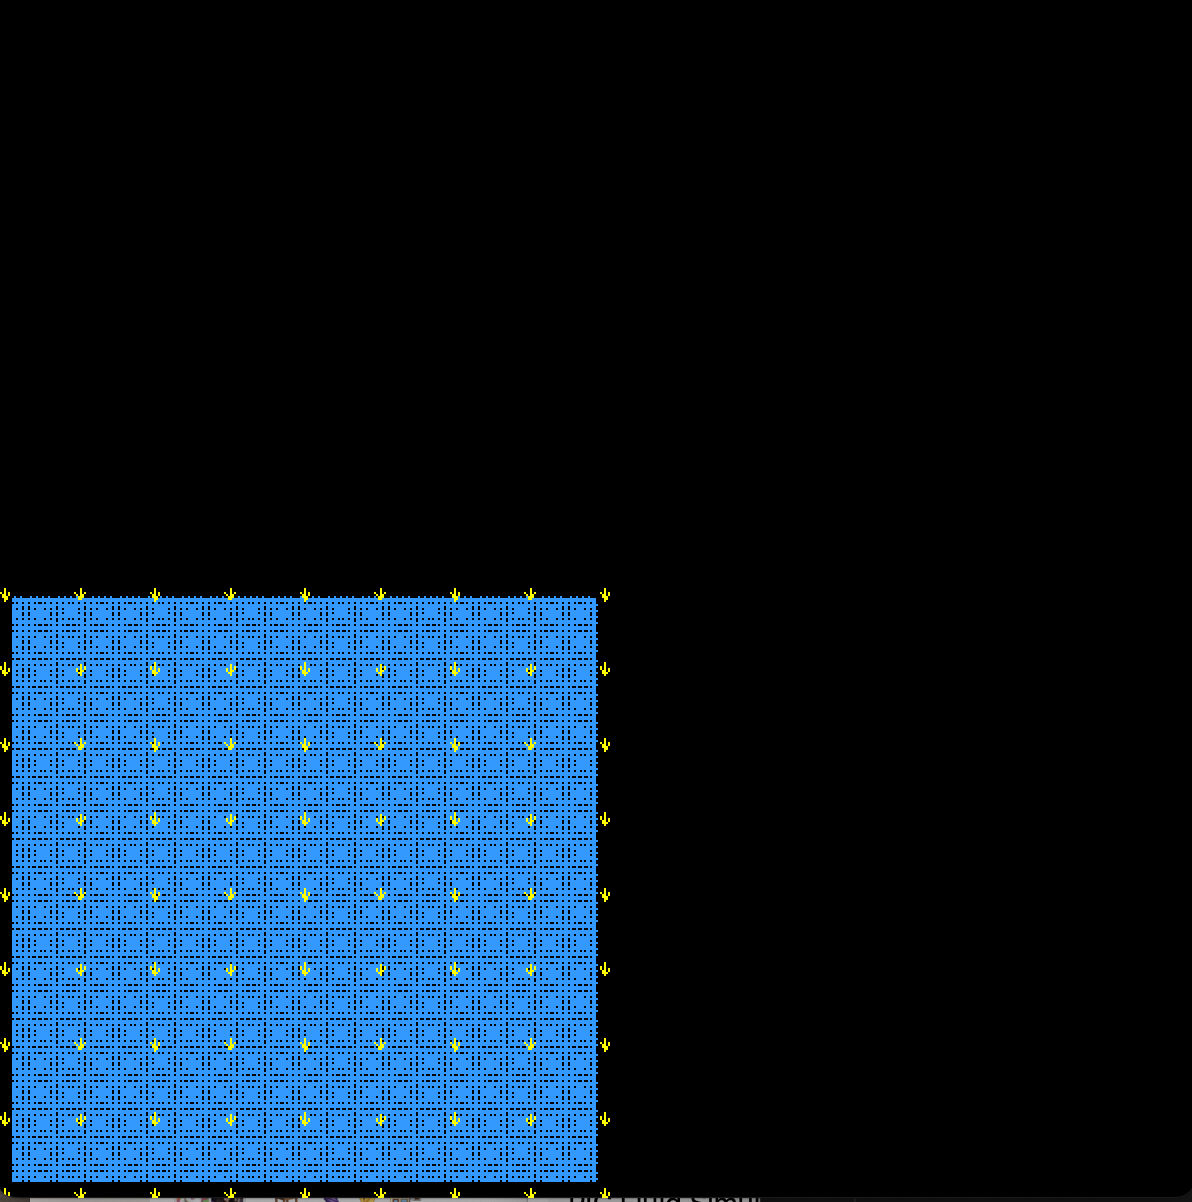
\includegraphics[width=\textwidth]{figures/pic_apply_g.png}
      \caption{After gravity is added, the grid velocity points downward.}
  \end{subfigure}
  \hspace{1em}
  \begin{subfigure}[t]{0.2\textwidth}
    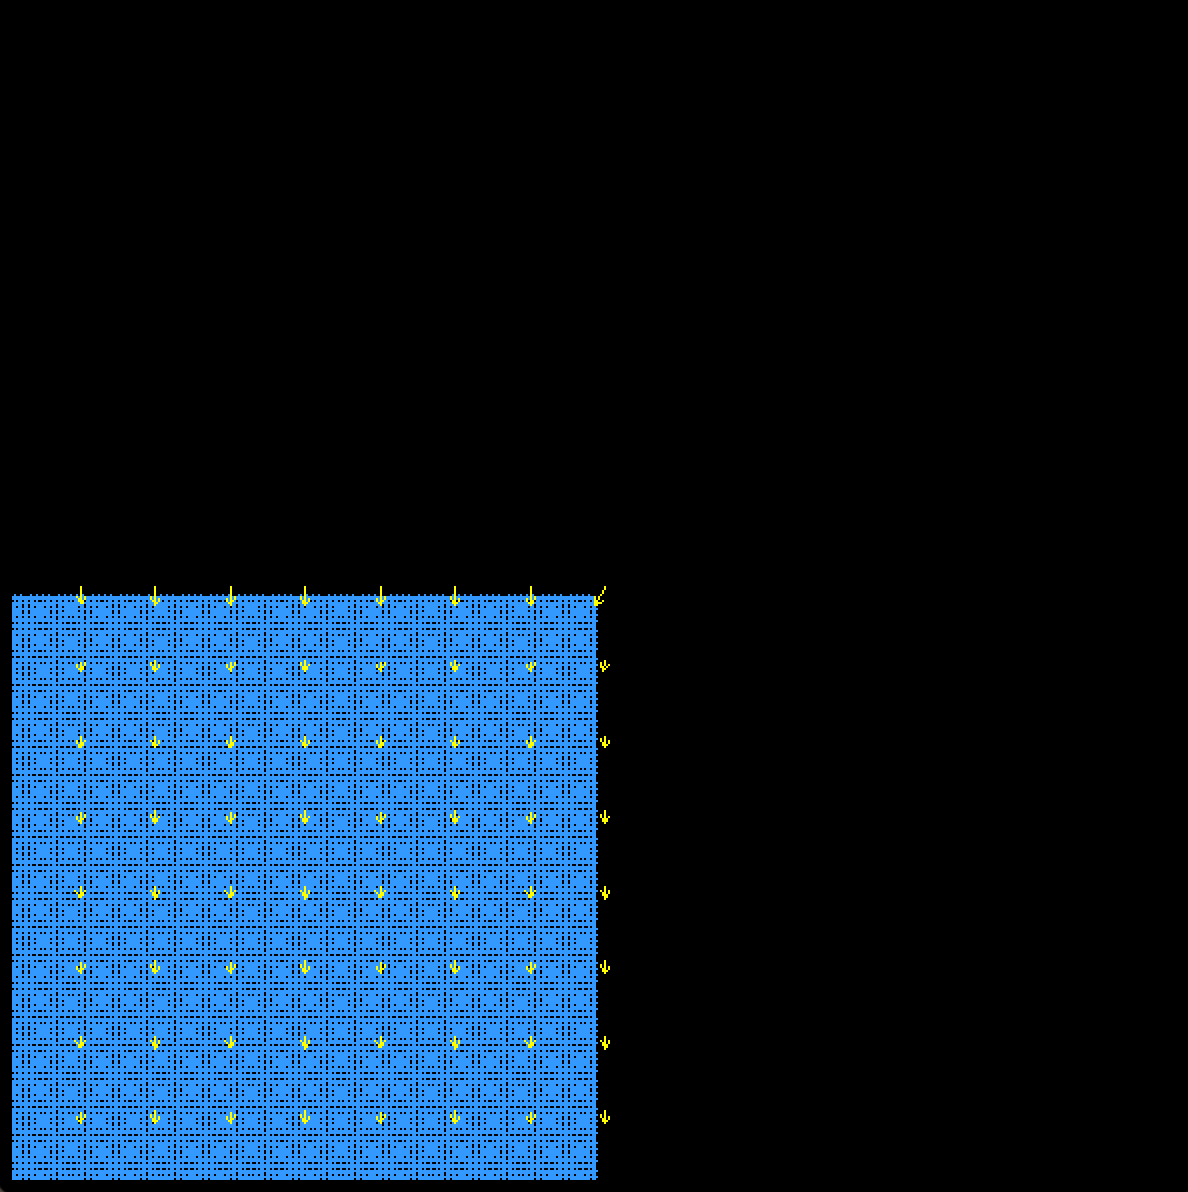
\includegraphics[width=\textwidth]{figures/pic_solve_pr.png}
    \caption{After solving pressure, the grid velocity becomes balanced.}
  \end{subfigure}
  \hspace{1em}
  \begin{subfigure}[t]{0.2\textwidth}
    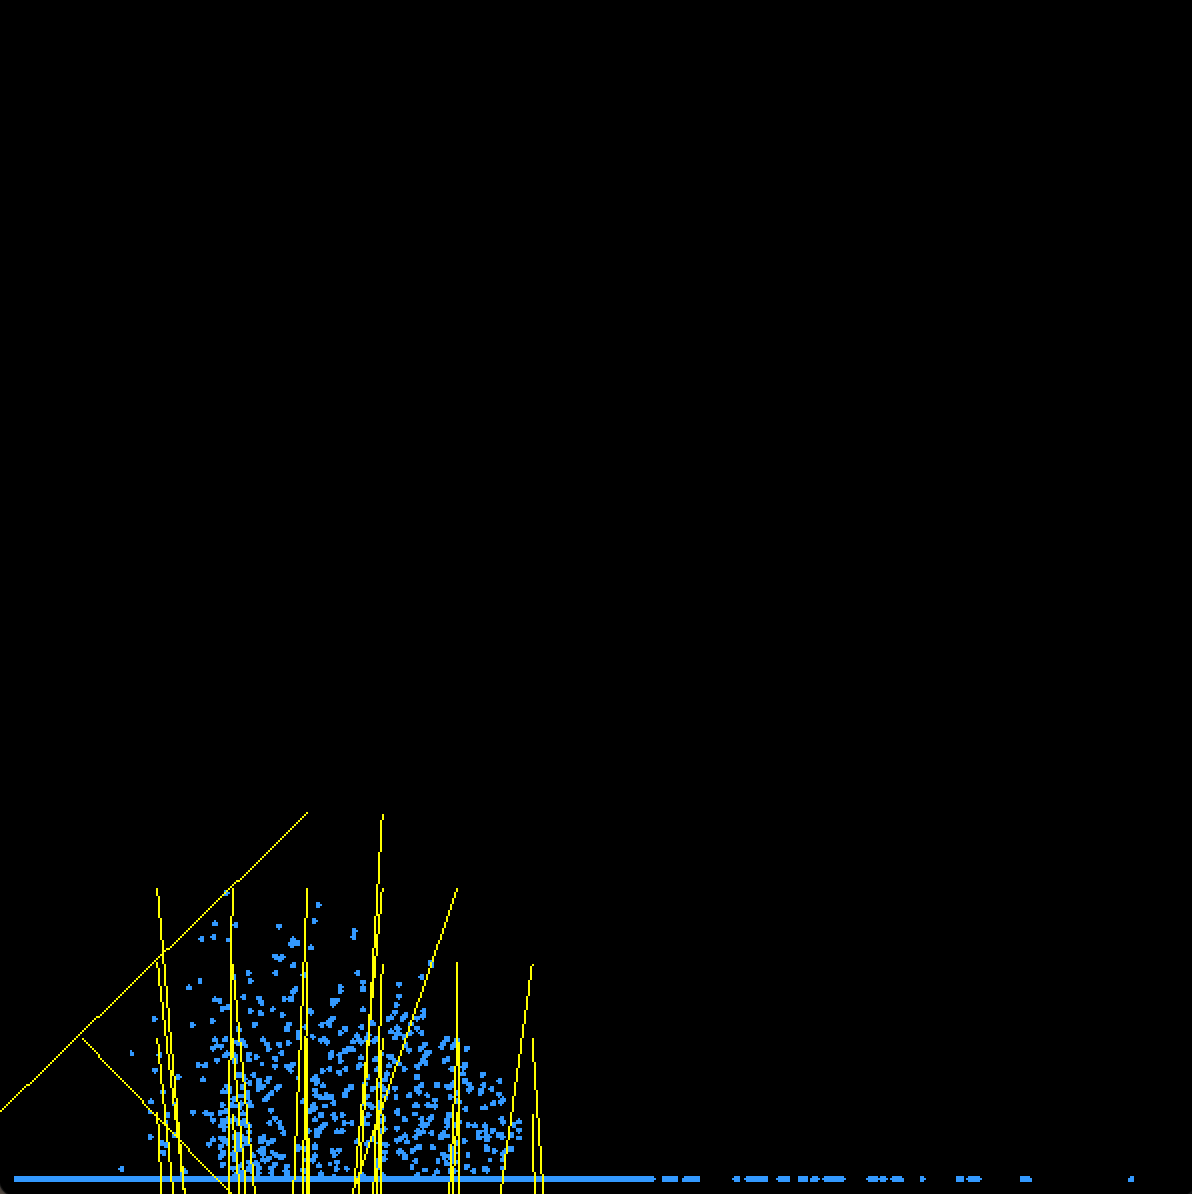
\includegraphics[width=\textwidth]{figures/pic_interm.png}
    \caption{Particles start to move after updating their velocity.}
  \end{subfigure}
  \caption{PIC simulation: Grid velocities update loop}
  \label{fig:pic}
\end{figure*}

\subsection{PIC/FLIP Implementation}

The PIC/FLIP hybrid method follows a similar pipeline but differs in how particle velocities are updated:

\begin{enumerate}
\item Before applying gravity, the current grid velocity is stored.

\item After solving the pressure, the difference between the new and old grid velocities is computed.

\item Particle velocities are updated using a blend of PIC and FLIP:
\begin{equation}
  \vec{v}_p^{blended} = \vec{v}_p^{PIC} + \alpha(\vec{v}_g^{new} - \vec{v}_g^{old})
  % \begin{aligned}
  % &\text{blended\_velocity} \\
  % &= \text{ particle\_velocity} \\
  % &+ \text{ flip\_ratio} \cdot (\text{new\_grid\_velocity} - \text{old\_grid\_velocity})
  %\end{aligned}
\end{equation}
where a flip\_ratio of 0 corresponds to pure PIC, and values approaching 1 resemble FLIP.

\item Particles are then advected in the same manner as the PIC method, including boundary handling.
\end{enumerate}

\subsubsection{Intermediate Results and Diagrams (PIC/FLIP)}


% \input{Sections/flip}
apic

% \section{Results}

\subsection{APIC}

We evaluated the performance of the APIC method with different particle counts. Figure~\ref{fig:apic_comparison} shows simulation snapshots at three resolutions—1000, 4000, and 8000 particles—demonstrating how the method handles fluid detail, stability, and distribution over time. Each subfigure compares the final state of the fluid, and highlights how increasing the number of particles leads to smoother, more detailed results.

\begin{figure*}[h]
    \centering
    \begin{subfigure}[b]{0.2\textwidth}
        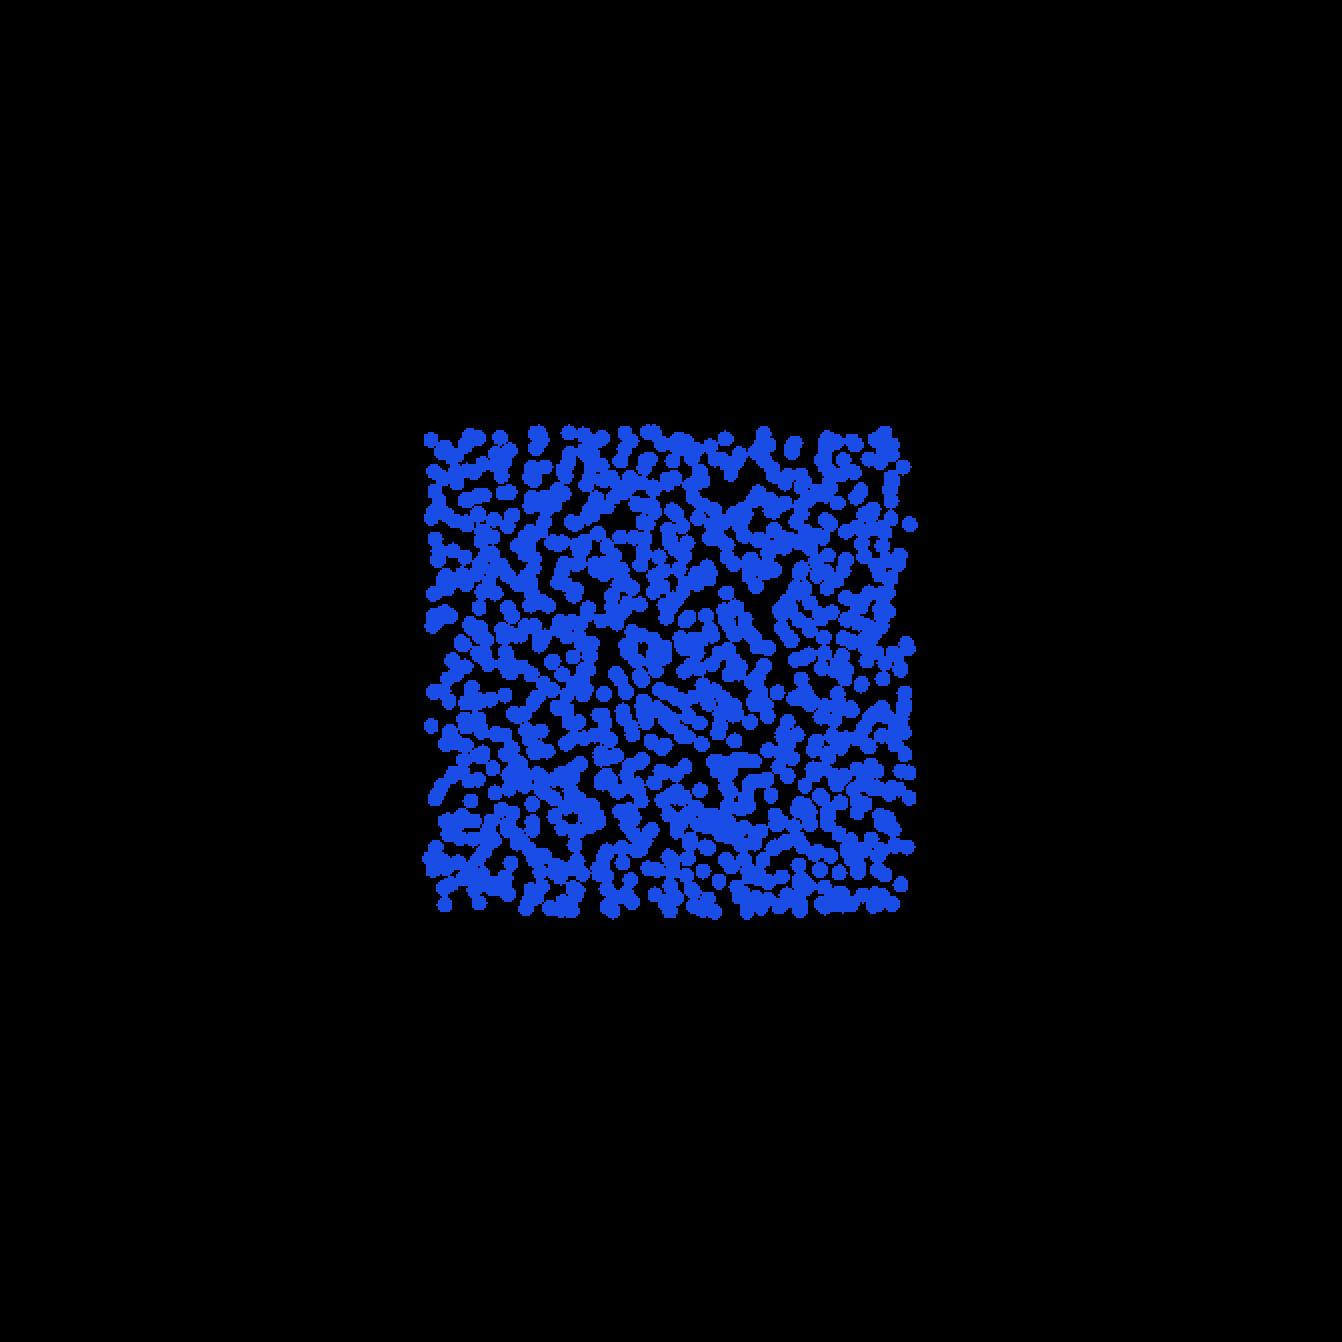
\includegraphics[width=\textwidth]{figures/apic1000_init.png}
        \caption{1000 initial particles}
    \end{subfigure}
    \begin{subfigure}[b]{0.2\textwidth}
        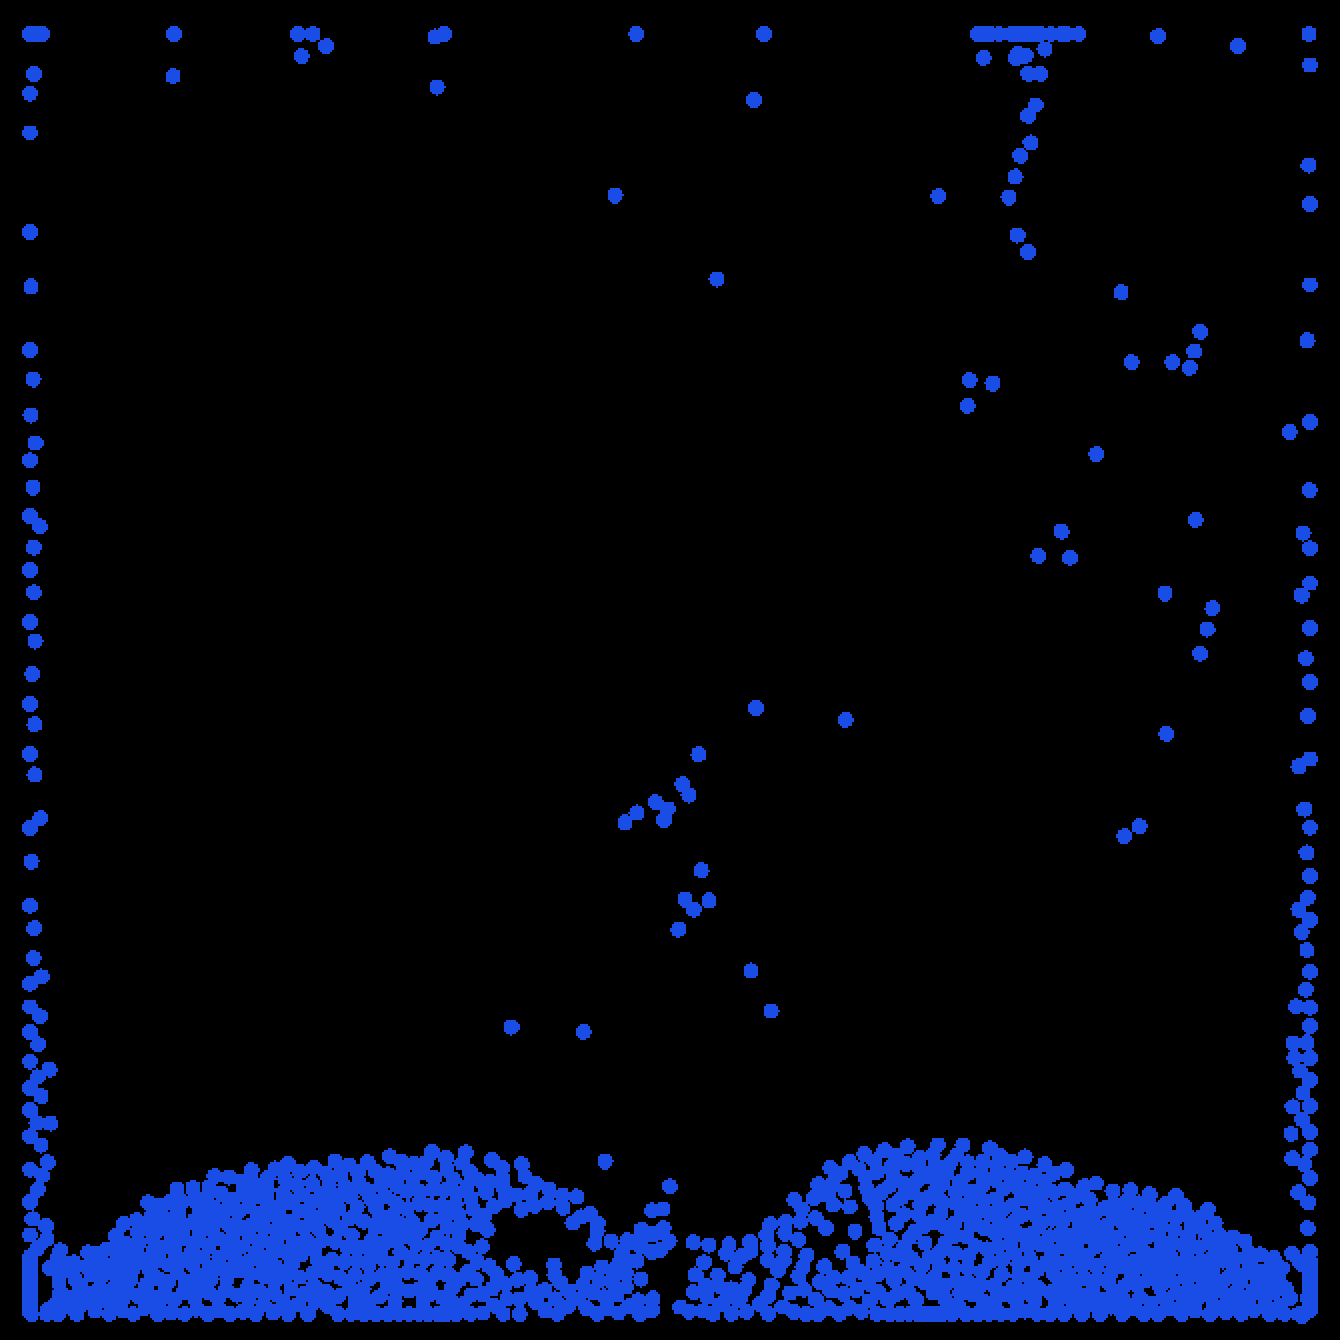
\includegraphics[width=\textwidth]{figures/apic1000.png}
        \caption{1000 particles}
    \end{subfigure}
    \begin{subfigure}[b]{0.2\textwidth}
        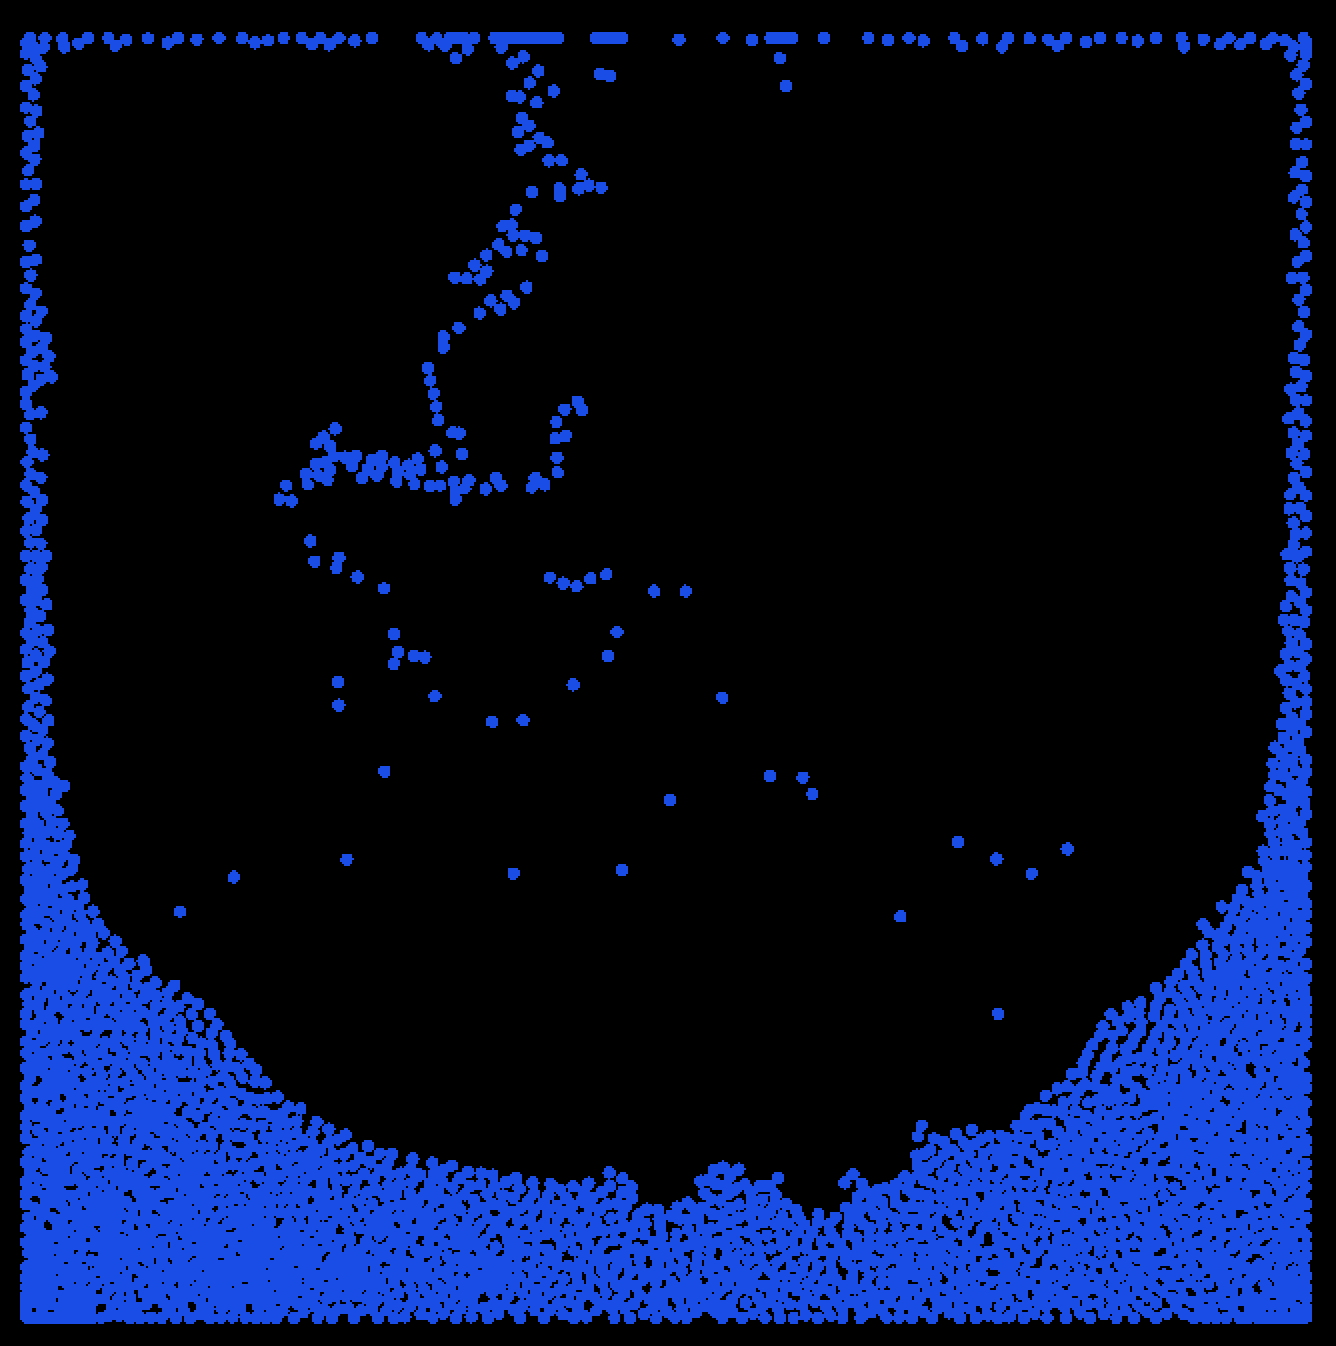
\includegraphics[width=\textwidth]{figures/apic4000.png}
        \caption{4000 particles}
    \end{subfigure}
    \begin{subfigure}[b]{0.2\textwidth}
        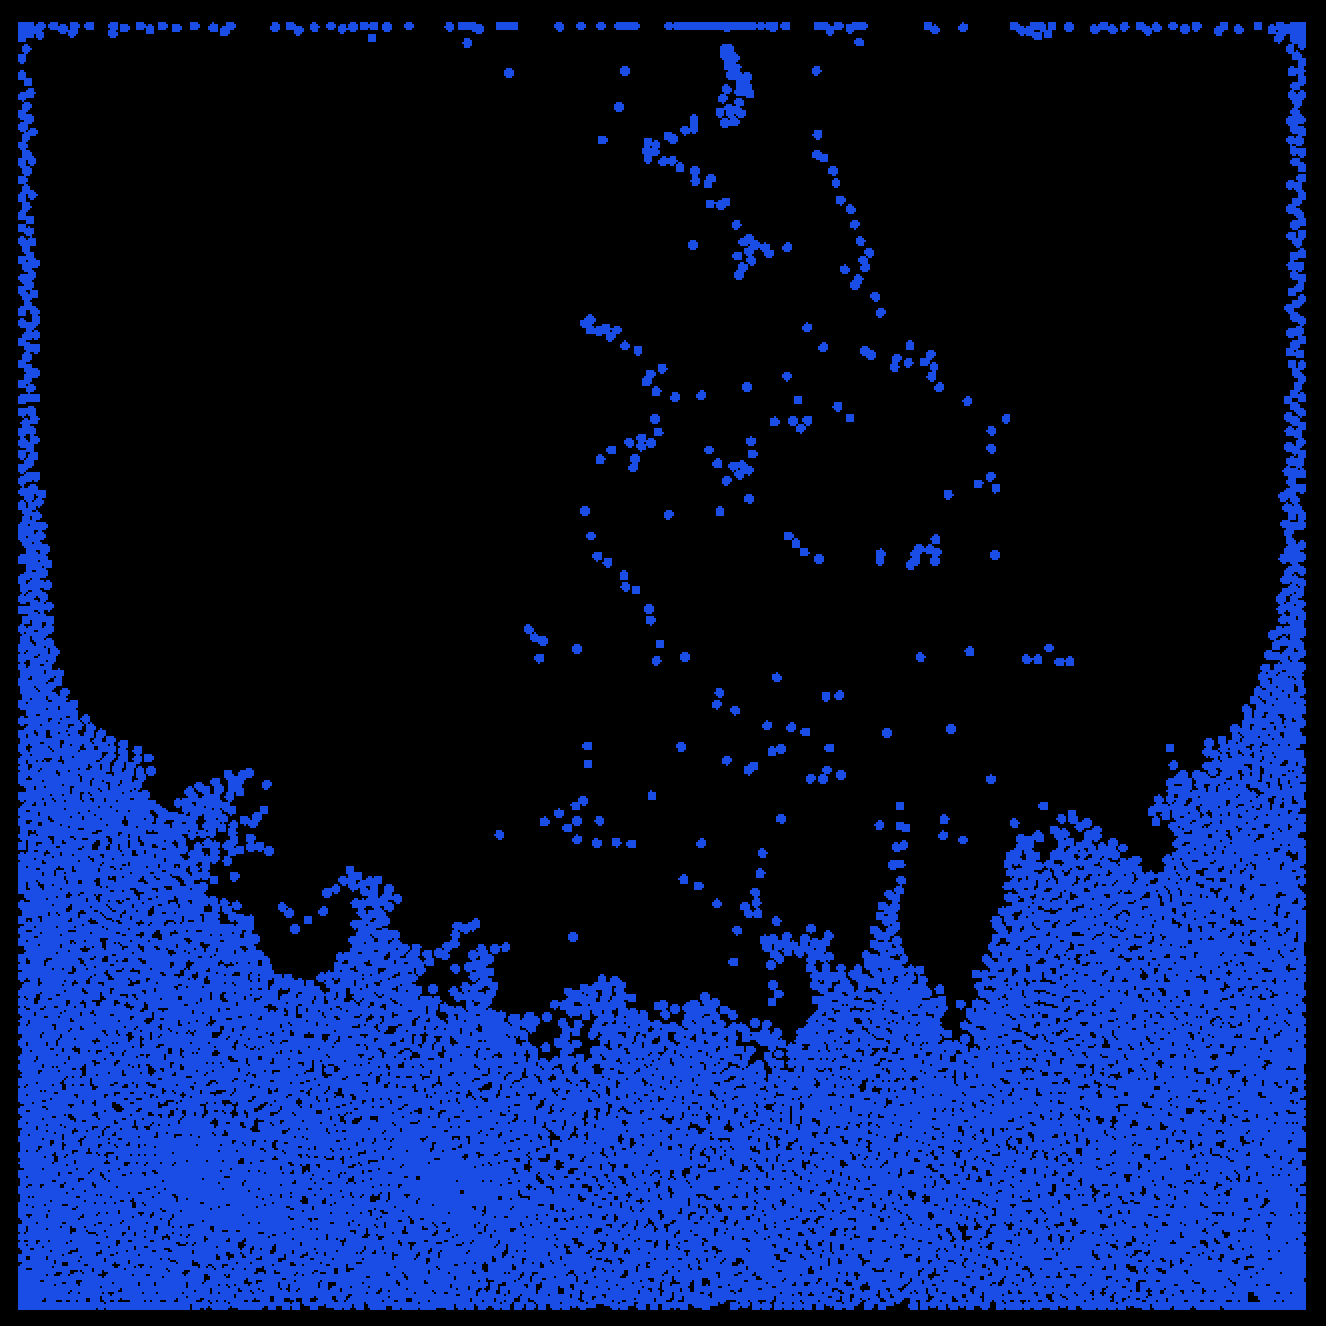
\includegraphics[width=\textwidth]{figures/apic8000.png}
        \caption{8000 particles}
    \end{subfigure}
    \caption{Comparison of APIC simulation results with increasing particle counts. 
    (a) shows the initial particle configuration, where all particles are placed in the center of the domain. 
    (b)–(d) show the simulation at the moment particles start to fall under gravity.}
    \label{fig:apic_comparison}
\end{figure*}
% \section{Discussion}
\subsection{Method Contributions}
\subsubsection{APIC}
The APIC method contributed most significantly to the visual quality of our simulations. By introducing an affine velocity field per particle, APIC preserves both rotational motion and local deformation, resulting in smoother, more detailed fluid behavior. Compared to PIC and FLIP, it produced the most visually stable and coherent results, especially at higher particle counts. The use of affine velocity transfer also reduced numerical dissipation and prevented particle clumping, leading to more realistic motion.

\subsection{Strengths}
\subsubsection{APIC}
APIC preserved rotational motion and fine detail better than other methods. It produced smooth and stable results even with 10000 particles. Compared to PIC and FLIP, it avoided both dissipation and noise, leading to visually realistic fluid behavior.

\subsection{Limitations}
\subsubsection{APIC}
APIC is computationally expensive due to affine matrix operations and additional interpolation. Performance drops at high particle counts, and the method becomes less suitable for real-time applications. It is also more complex to implement than PIC or FLIP, requiring careful handling of matrix math, boundary conditions, and velocity transfers to avoid instability.
% \section{Conclusion}
 
Through this project, we gained hands-on experience implementing a variety of fluid simulation methods, including particle-based (SPH), grid-based (Stable Fluids), and hybrid approaches (PIC, FLIP, and APIC). We deepened our understanding of pressure projection, velocity interpolation, particle-grid transfers, and fluid behavior visualization. On the implementation side, we learned to work with OpenGL and GLUT for real-time rendering, and used the Eigen library for efficient linear algebra operations. We also practiced debugging and tuning numerical simulations, and managing complexity within a modular C++ codebase.

\textbf{Team Contributions}   Xu Chen was responsible for the OpenGL-based visualization system and implemented the APIC method. Yumeng He contributed to both the particle system and grid-based simulation components. Irene Li worked on particle and grid simulations. Yuchen Chen implemented the PIC and FLIP methods and also contributed to grid development.

\textbf{Future Work }   This project has sparked our interest in computer graphics and physically based animation. In the future, we hope to explore more advanced topics such as 3D fluid simulation, GPU acceleration, and real-time rendering techniques.

\section*{Acknowledgements}
This project received support during the CSCI580 course, instructed by Professor XXX at the University of Southern California, USA.

\printbibliography

\end{document}
